% Use only LaTeX2e, calling the article.cls class and 12-point type.

\documentclass[12pt]{article}

%Cosas copiadas del paper de Iñigo
\usepackage[table]{xcolor}
\RequirePackage{siunitx}
\RequirePackage[T1]{fontenc}                        % T1 font encoding for PDFs
\RequirePackage{lmodern}                                % extended font definition
\RequirePackage{amsmath,amssymb,amsthm} % most important math stuff
\RequirePackage{a4wide}                                 % make better use of A4 paper
\RequirePackage{fancyhdr}                               % custom headers and footers
\RequirePackage{fncychap}                               % custom chapter titles
\RequirePackage{graphicx}                               % graphics
\RequirePackage{color}                                  % color
\RequirePackage{booktabs}                               % extra tabular commands
\RequirePackage[format=plain]{caption}  % improved caption format
\RequirePackage{nomencl}                                % cool nomenclature listing
\RequirePackage{makeidx}                                % create your index
\RequirePackage[printonlyused]{acronym}
\RequirePackage{ifthen}                                 % if-then commands (used in maketitle)
\RequirePackage{eso-pic}                                % picture in back/forground (used in cover)
\RequirePackage{relsize}                                % \textlarger, \textsmaller etc
%%
%%
%%%%%%%%%%%%%%%%%%%%%%%%%%%%%%%%%%%%%%%%%%%%%%%%%%%%%%%%%%%%
%%
%%  Set up Matlab and C++ Listings
%%  REQUIRES PACKAGE listings AND colortbl
%%
%%%%%%%%%%%%%%%%%%%%%%%%%%%%%%%%%%%%%%%%%%%%%%%%%%%%%%%%%%%%
%%
%%

\RequirePackage{listings}%

\usepackage[utf8]{inputenc}

\usepackage{pgf,tikz}

\usepackage{pgfgantt}

\usepackage{mathrsfs}

\usepackage{mathtools}

\usepackage{gensymb}

\usepackage{float}

\usepackage{needspace}

\usepackage{pgfplots}

\usepackage[nodayofweek,level]{datetime}

\usepackage{todonotes}

\usepackage{bm}

\usepackage{enumitem}

\usepackage{graphicx}

\usepackage{subcaption}

\usepackage{indentfirst}

\usepackage{multirow}

\usepackage{eurosym}

\usepackage{hhline}

\usepackage{esvect}


\usepackage{upgreek}
\usepackage{arydshln}
\usepackage{algorithm}
\usepackage[noend]{algpseudocode}

\usepackage[nameinlink,capitalise]{cleveref}

\usepackage{mathtools}
%%%%%%%%%%% COPYPASTEADO DE GITHUB
\usepackage{amsmath}
\usepackage{amssymb}

\usepackage{wrapfig}

%redefine vector and Real symbols for faster typing
\renewcommand{\vec}[1]{\bm{#1}}
\newcommand{\R}{\mathbb R}
\newcommand{\Z}{\mathbb Z}
\newcommand{\foralli}[1][]{\forall i \in \{1\dots n_{#1}\}}
\newcommand{\forallj}[1][]{\forall j \in \{1\dots n_{#1}\}}
\newcommand{\forallk}[1][]{\forall k \in \{1\dots n_{#1}\}}
\newcommand{\dd}[2]{\frac{\partial #1}{\partial #2}}
\newcommand{\dt}[1]{\frac{d #1}{d t}}
\newcommand{\torque}{\tau}
\newcommand{\w}{\dot\varphi}
\newcommand{\h}{\frac{1}{2}}
\newcommand{\pare}[1]{\left(#1\right)}
\newcommand{\brac}[1]{\left\{#1\right\}}

\newcommand{\mat}[2][b]{\begin{#1matrix}#2\end{#1matrix}}

%set spacing between rows in tables
\renewcommand{\arraystretch}{1.2}

\def\F{\vec F}
\def\Torque{\vec \Gamma}
\def\R{\vec R}

\def\q{\vec q}
\def\M{\vec M}
\def\I{\vec I}
\def\C{\vec C}
\def\mults{\vec \lambda}

%   Fin de la parte copypasteada
\graphicspath{ {images/} }

% Users of the {thebibliography} environment or BibTeX should use the
% scicite.sty package, downloadable from *Science* at
% www.sciencemag.org/about/authors/prep/TeX_help/ .
% This package should properly format in-text
% reference calls and reference-list numbers.

\usepackage{scicite}

% Use times if you have the font installed; otherwise, comment out the
% following line.

\usepackage{times}

% The preamble here sets up a lot of new/revised commands and
% environments.  It's annoying, but please do *not* try to strip these
% out into a separate .sty file (which could lead to the loss of some
% information when we convert the file to other formats).  Instead, keep
% them in the preamble of your main LaTeX source file.


% The following parameters seem to provide a reasonable page setup.

\topmargin 0.0cm
\oddsidemargin 0.2cm
\textwidth 16cm 
\textheight 21cm
\footskip 1.0cm


%The next command sets up an environment for the abstract to your paper.

\newenvironment{sciabstract}{%
\begin{quote} \bf}
{\end{quote}}


% If your reference list includes text notes as well as references,
% include the following line; otherwise, comment it out.

\renewcommand\refname{References and Notes}

% The following lines set up an environment for the last note in the
% reference list, which commonly includes acknowledgments of funding,
% help, etc.  It's intended for users of BibTeX or the {thebibliography}
% environment.  Users who are hand-coding their references at the end
% using a list environment such as {enumerate} can simply add another
% item at the end, and it will be numbered automatically.

\newcounter{lastnote}
\newenvironment{scilastnote}{%
\setcounter{lastnote}{\value{enumiv}}%
\addtocounter{lastnote}{+1}%
\begin{list}%
{\arabic{lastnote}.}
{\setlength{\leftmargin}{.22in}}
{\setlength{\labelsep}{.5em}}}
{\end{list}}


% Include your paper's title here

\title{Considerations on Acceleration, Forces and Electric Power of the Omnibot} 


% Place the author information here.  Please hand-code the contact
% information and notecalls; do *not* use \footnote commands.  Let the
% author contact information appear immediately below the author names
% as shown.  We would also prefer that you don't change the type-size
% settings shown here.

\author
{Siro Moreno$^{1\ast}$ \\
\\
\normalsize{$^{1}$Institut de Robótica i Informática Industrial}\\
\normalsize{dirección del IRI, Barcelona}\\
\normalsize{$^\ast$To whom correspondence should be addressed; E-mail:  ejemplo@ejemplo.eje}
}

% Include the date command, but leave its argument blank.

\date{}



%%%%%%%%%%%%%%%%% END OF PREAMBLE %%%%%%%%%%%%%%%%



\begin{document} 

% Double-space the manuscript.

\baselineskip24pt

% Make the title.

\maketitle 



% Place your abstract within the special {sciabstract} environment.

\begin{sciabstract}
  We will discuss some considerations and insights of the relationships between forces, accelerations and electric power using the alternative axes of the Omnibot robot previously discussed.
\end{sciabstract}



% In setting up this template for *Science* papers, we've used both
% the \section* command and the \paragraph* command for topical
% divisions.  Which you use will of course depend on the type of paper
% you're writing.  Review Articles tend to have displayed headings, for
% which \section* is more appropriate; Research Articles, when they have
% formal topical divisions at all, tend to signal them with bold text
% that runs into the paragraph, for which \paragraph* is the right
% choice.  Either way, use the asterisk (*) modifier, as shown, to
% suppress numbering.

\section*{Motors electric models and their meaning}

\begin{center}
	\begin{tabular}{ | m{12em} | m{10em}| } 
		\hline
		Complete model & Simplified model \\ 
		\hline
		$$ V = K_m N\dot{\phi} + Ri$$
		$$ \tau_m = N K_ei\mu_{trans} - \tau_r$$
		$$ \tau_r = a \dot{\phi} + b \operatorname{sign}(\dot{\phi}) $$ &
		$$ V = K_m N\dot{\phi} + Ri$$
		$$ \tau_m = N K_ei$$ \\ 
		\hline
	\end{tabular}
\end{center}
On the first column we have the electric motor model as we have been using it. It includes the effects of friction and transmission losses up to the wheel shaft. On the right we have a simplified model, that drops the transmission efficiency and friction, but keeps the electrical resistance. The reason to use this model is that we want to separate the dissipative effects that are due friction from those that are intrinsic to electric motors, and compare them to get a better understanding of the nature of the model.

We can easily obtain that:
$$P_{e, simp} = Vi = \frac{K_{m} \tau_{m} \dot{\phi}}{K_{e}} + \frac{R_{e} \tau_{m}^{2}}{K_{e}^{2} N^{2}}$$

We can observe that if we were to consider a perfect motor where resistance was zero and $K_e = K_m$, the electric power would collapse back to $P = Vi = \tau_{m} \dot{\phi}$, a perfect conversion of electricity into mechanic power. Since we have already studied the robot's mechanics without motors, no additional insight would be obtained. Thus, we are keeping the electrical losses. We can substitute the parameters with their values for additional clarity:

$$ P_{e, simp} = 0.677 \tau_{m}^{2} + 0.934 \tau_{m} \dot{\phi}$$

The equivalent expression with the complete model is more complex, but it is worth showing for the sake of symmetry:
$$ P_{e,comp} = 1.881 \tau_{m}^{2} + 1.505 \tau_{m} \operatorname{sign}\left(\dot{\phi}\right) + \left(1.594 \tau_{m} + 0.638 \operatorname{sign}\left(\dot{\phi}\right)\right) \dot{\phi} + 0.301 \operatorname{sign}^{2}\left(\dot{\phi}\right) + 0.016 \dot{\phi}^{2}$$

We can see that both expressions are functions only of $\tau_{m}$ and $\dot{\phi}$, so it will be interesting to plot them in a 2d graph of both magnitudes as axes. In order to plot only valid values, we need to calculate the envelope of achievable values, that is, maximum and minimum torque at a certain  $\dot{\phi}$. We do so by substituting the value of $V$ by its maximum and minimum value. We are interested in behaviour obtainable in normal conditions, so we will limit our graph in $\dot{\phi}$ only up to the maximum speed that the motor can achieve by itself. Since the expression is symmetric, we can start our graph at zero speed.
\begin{figure}[h]
	\centering
	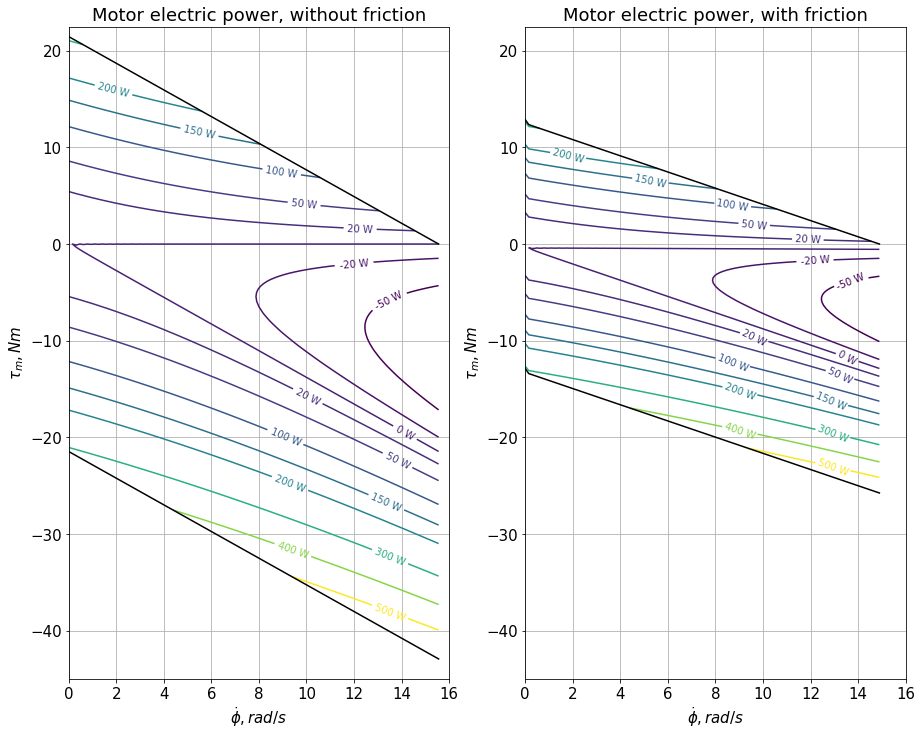
\includegraphics[width=.5\linewidth]{motor_electric_power_w_and_wout_fricc}
	\captionof{figure}{power as function of torque and speed}
	\label{fig:power_f_tau_speed}
\end{figure}

Just at first sight we can spot some differences between the two graphs. The main difference is that without friction, the achievable torque is almost double, in both signs. The maximum speed achievable is slightly decreased, but the electric power looks scaled with the torque, so its limit values are not that different.

We can also see some very interesting features on this graph. Lets start with the lines where $P = 0$. 

The horizontal one, which overlaps with the zero torque axe in the no friction graph, represents the condition where $i = 0$. It is easy to understand that the electric power is zero, because it is equivalent of having a motor with its terminals disconnected. In the complete model graph, this line is also present but slightly under the axe, as it shows the friction acting as a small breaking torque.

We have another line of power zero, this time diagonal, and always equidistant from the maximum and minimum torque at any $\dot{\phi}$. This line corresponds to $V = 0$, and is also easy to understand that the electric power spent there is zero, as it is equivalent to have a motor with its terminals connected with each other.

Between them, we have a triangular area where the power is negative, that is, the motor is acting as generator. While it is expected in the simplified case, we have to be very cautious when using the complete expression. The most obvious problem we encounter is that the torque efficiency $\mu_{trans}$ is defined when the motor is driving the wheel but not the opposite! Without further testing, it is difficult to know if its value would flip to its inverse or even decay to infinite because of imposibility to run the transmission backwards, as in a worm gear. My suggestion in this case would be to take a value of zero when a negative power is calculated.
\begin{center}
	\begin{tabular}{ | m{14em} | } 
		\hline
		Modified model \\ 
		\hline
		$$ V = K_m N\dot{\phi} + Ri$$
		$$ \tau_m = N K_ei\mu_{trans} - \tau_r$$
		$$ \tau_r = a \dot{\phi} + b \operatorname{sign}(\dot{\phi}) $$
		$$ P_{e}=\begin{cases}
		Vi \text{  if  } Vi\geq 0\\
		0 \text{  if  } Vi < 0
		\end{cases}$$\\
		
		\hline
	\end{tabular}
\end{center}


\section*{Application to the complete robot model}

We remember that the complete model projected on axes 2 is:
$$\vec{H} \vec a+\vec K\vec w=\R^T\vec\Gamma$$
We can explore how the proposed motor models interact with the robot model in different conditions.

\subsection*{Envelope of achievable accelerations}
If we express acceleration as a function of $\Gamma$ and $\vec w$:
$$ \vec a = \left[\begin{matrix}a_{1}\\a_{2}\\\ddot{\psi}\end{matrix}\right] = \vec H^{-1}(\R^T \vec \Gamma - \vec K \vec w) =  \left[\begin{matrix}\frac{- 4 I_{w} w_{2} \dot{\psi} + \sqrt{2} r \left(\tau_{1} + \tau_{4}\right)}{4 I_{w} + m r^{2}}\\\frac{4 I_{w} w_{1} \dot{\psi} + \sqrt{2} r \left(\tau_{2} + \tau_{3}\right)}{4 I_{w} + m r^{2}}\\- \frac{\sqrt{2} L_{2} r \left(\tau_{1} - \tau_{2} + \tau_{3} - \tau_{4}\right)}{8 I_{w} L_{2}^{2} + I_{z} r^{2}}\end{matrix}\right]$$

We can observe some interesting details:
\begin{itemize}
	\item As we expected, acceleration in direction $a_1$ only depends on $\tau_1$ and $\tau_4$, while in direction $a_2$ only on $\tau_2$ and $\tau_3$. This means that when representing the envelope of achievable accelerations for any given condition, it will always be a rectangle.
	\item Maximum acceleration in direction $a_1$ is achieved with maximum $\tau_1$ and $\tau_4$, that is, with maximum voltage on those motors, and equivalent for minimum acceleration. The same logic applies to $a_2$. This means that we can easily calculate its extreme values by substituting maximum or minimum values of voltage in the motor models.
\end{itemize}
\subsection*{No rotation condition}
When $\dot\psi = 0, \vec K =\vec 0$:
$$ \vec H\vec a = \R^T\vec \Gamma$$
$$\vec \Gamma = \R^{-1T}\vec H\vec a = \frac{\sqrt{2} r \left(\frac{4 I_{w}}{r^{2}} + m\right)}{4}\left[\begin{matrix}a_{1} \\a_{2} \\a_{2} \\a_{1} \end{matrix}\right]$$
$$\dot{\q_w} = \R \vec{w} = \frac{\sqrt{2}}{r} \left[\begin{matrix}w_1\\w_2\\w_2\\w_1\end{matrix}\right]$$

For each motor we can calculate the power as a function of $\tau$ and $\dot\phi$, and we saw how they can be expressed in terms of $\vec a$ and $\vec w$. Adding the power of the four motors, we get the total power.

Doing so, we can get readable formulas for the simplified and complete model, but not for the modified model, where we will switch to a numeric approach:
$$P_{e, simp} = 0.25 a_{1}^{2} + 16.95 a_{1} w_{1} + 0.25 a_{2}^{2} + 16.95 a_{2} w_{2}$$
$$P_{e, comp} = 0.69 a_{1}^{2} + 1.29 a_{1} \operatorname{sign}\left(w_{1}\right) + 0.69 a_{2}^{2} + 1.29 a_{2} \operatorname{sign}\left(w_{2}\right) + 14.17 w_{1}^{2} +$$
$$+ 42.41 w_{1} \left(0.68 a_{1} + 0.64 \operatorname{sign}\left(w_{1}\right)\right) + 14.17 w_{2}^{2} + 42.41 w_{2} \left(0.68 a_{2} + 0.64 \operatorname{sign}\left(w_{2}\right)\right) +$$
$$+ 0.6 \operatorname{sign}^{2}\left(w_{1}\right) + 0.6 \operatorname{sign}^{2}\left(w_{2}\right)$$
\subsubsection*{Envelope of accelerations}
For both models, simple and complete, we can find an expression that give the value of torque as a function of the speed and the voltage:
$$\tau_{simp} = \displaystyle - \frac{K_{e} K_{m} N^{2} \dot{\phi}}{R_{e}} + \frac{K_{e} N V}{R_{e}} \approx 0.894 V - 1.38 \dot{\phi}$$
$$\tau_{comp} = - \frac{K_{e} K_{m} N^{2} \mu \dot{\phi}}{R_{e}} + \frac{K_{e} N V \mu}{R_{e}} - a \dot{\phi} - b \operatorname{sign}\left(\dot{\phi}\right)\approx 0.537 V - 0.4 \operatorname{sign}\left(\dot{\phi}\right) - 0.838 \dot{\phi}$$

We can substitute in these expressions the value of V with it maximum (24V), minimum (-24V) and zero values, in order to get maximum, minimum and zero-voltage torques as functions of $\dot \phi$. We can then get arrays for maximum, minimum and zero-voltage $\Gamma$ as functions of $\vec w$. Then, using
$$\vec a = \vec H^{-1} \R^{T} \vec \Gamma$$ 
We can obtain values for maximum, minimum and zero-voltage accelerations:
$$\vec a_{simp, max} \approx \left[\begin{matrix}50.178 - 68.379 w_{1}\\50.178 - 68.379 w_{2}\\0\end{matrix}\right], \  \vec a_{simp, min} \approx \left[\begin{matrix}- 68.379 w_{1} - 50.178\\- 68.379 w_{2} - 50.178\\0\end{matrix}\right], \  \vec a_{simp, 0V} \approx \left[\begin{matrix}- 68.379 w_{1}\\- 68.379 w_{2}\\0\end{matrix}\right]$$
$$\vec a_{comp, max} \approx \left[\begin{matrix}- 41.523 w_{1} - 0.935 \operatorname{sign}\left(w_{1}\right) + 30.107\\- 41.523 w_{2} - 0.935 \operatorname{sign}\left(w_{2}\right) + 30.107\\0\end{matrix}\right]$$
$$\vec a_{comp, min} \approx  \left[\begin{matrix}- 41.523 w_{1} - 0.935 \operatorname{sign}\left(w_{1}\right) - 30.107\\- 41.523 w_{2} - 0.935 \operatorname{sign}\left(w_{2}\right) - 30.107\\0\end{matrix}\right], \ \vec a_{comp, 0V} \approx   \left[\begin{matrix}- 41.523 w_{1} - 0.935 \operatorname{sign}\left(w_{1}\right)\\- 41.523 w_{2} - 0.935 \operatorname{sign}\left(w_{2}\right)\\0\end{matrix}\right]$$

We can observe than in both models, $a_{1,max} - a_{1,min} = a_{2,max} - a_{2,min} = C_{model}$, being $C_{model}$ a constant value different in each model. We can also see that the zero-voltage value is always the mean value between the maximum and the minimum. This means, as we will see in the graphs, that the envelope of achievable accelerations will always be a square of side $C_{model}$, centered on $\vec a_{0V}$.
\subsubsection*{Movement in one axis}
Let's start with a simple case where $w_2$ and $a_2$ are zero. In this case, only motors 1 and 4 work, and both run at the same speed and equal force. We can plot the electric power needed to achieve a certain acceleration while moving at a given speed, and we will see that it is the same graph as the motor alone, but with the power doubled since we now have two motors running.

\begin{figure}[h]
	\centering
	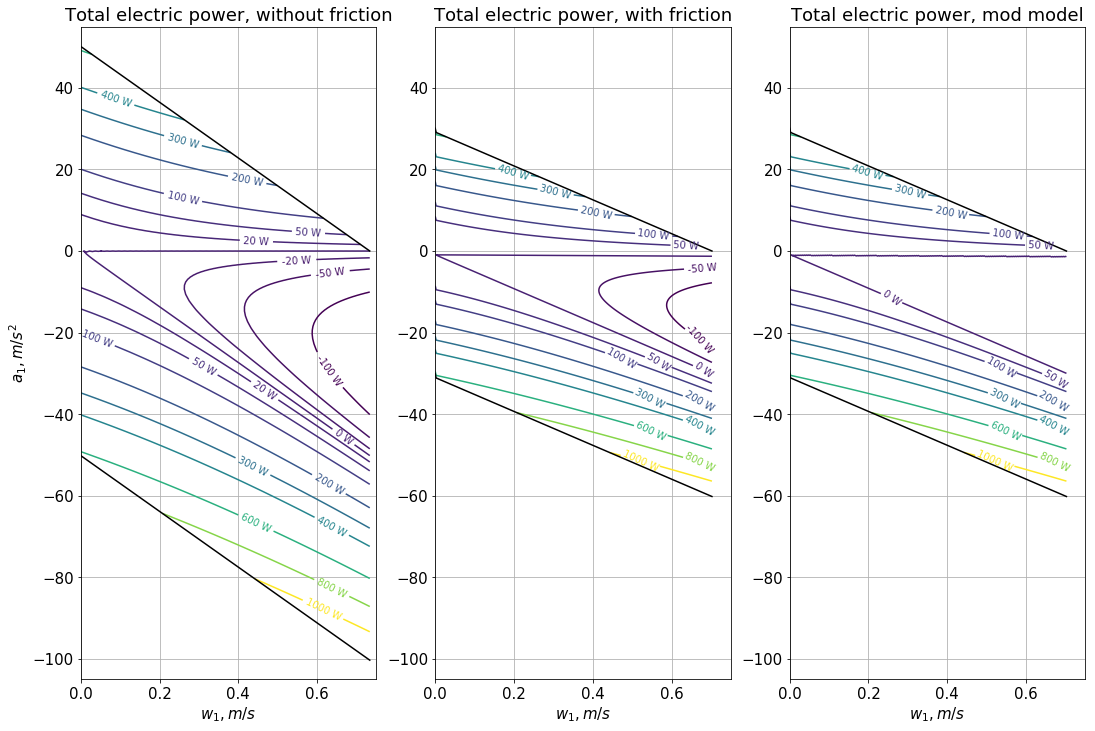
\includegraphics[width=.8\linewidth]{total_electric_power_w_and_wout_fricc}
	\captionof{figure}{power as function of acceleration and speed}
	\label{fig:power_f_a1_w1}
\end{figure}

\subsubsection*{Acceleration from static}
Let's suppose that we are static $\vec{w} = \vec{0}$ and want to get an acceleration. Substituting in the general no rotation expressions, we get:
$$P_{e, simp} = 0.25 a_{1}^{2} + 0.25 a_{2}^{2}$$
$$P_{e, comp} = 0.69 a_{1}^{2} + 0.69 a_{2}^{2}$$

We can see that in both cases, power required to accelerate scales with the acceleration module squared, independent from the direction. The modified model is equal to the complete model because there is no condition with negative power in the envelope of feasible accelerations.
\begin{figure}[h]
	\centering
	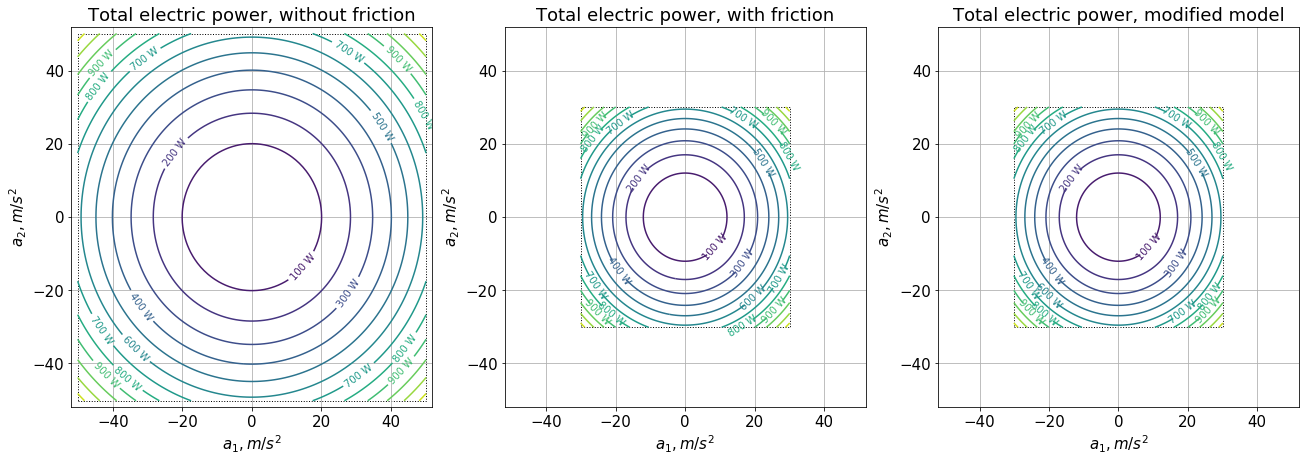
\includegraphics[width=1\linewidth]{power_from_static}
	\captionof{figure}{power as function of acceleration, from static}
	\label{fig:power_from_static}
\end{figure}

\subsubsection*{Moving at half speed in $w_1$}
As a second example, let's repeat the analysis but supposing the robot is moving at half its maximum speed in the direction of $w_1$.
\begin{figure}[h]
	\centering
	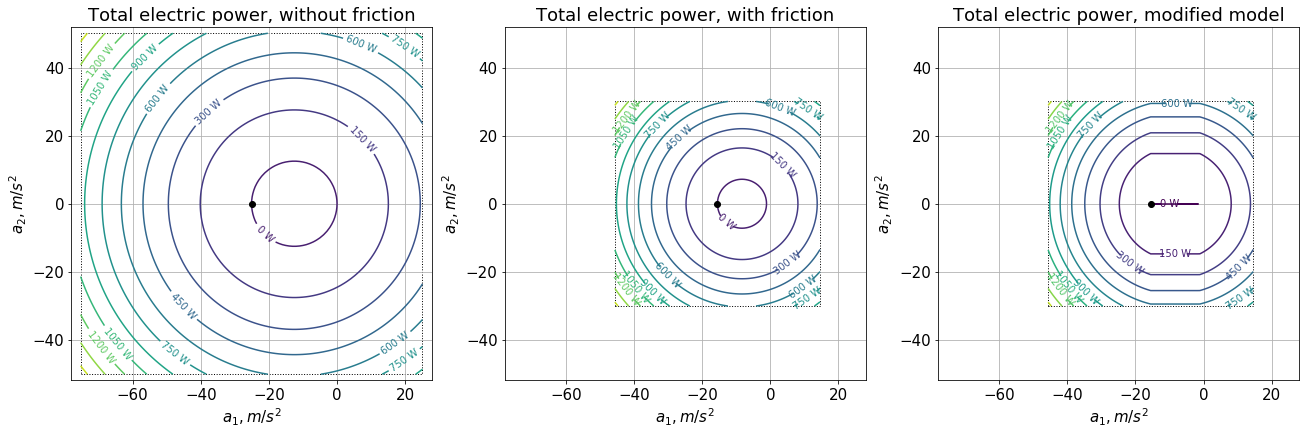
\includegraphics[width=1\linewidth]{power_from_w1}
	\captionof{figure}{power as function of acceleration, moving in $w_1$}
	\label{fig:power_from_w1}
\end{figure}
We can see that in the three graphs, the size of the square envelope of achievable accelerations remains unchanged, but its center is displaced to the point that corresponds to switching all voltages to zero.

Since we are moving with pure $w_1$ speed, the motors 1 and 4 have a range of torques where they could generate power (in the models that allow it). In the simple and complete models, we can observe it as a circular region that appears where power is negative, that is, where more power is generated in a pair of motors than spent in the other two.

In the modified model, as expected, that region collapses in a line. We can observe a rectangular area is created between the two $a_1$ values that limit where the power of motors 1 and 4 are zero. Since in that region of the map the power only depends on $a_2$, the lines become horizontal.

\subsubsection*{Moving at half speed in both $w_1$ and $w_2$}
As a third example, let's repeat the analysis but supposing the robot is moving at half its maximum speed in both directions.

\begin{figure}[h]
	\centering
	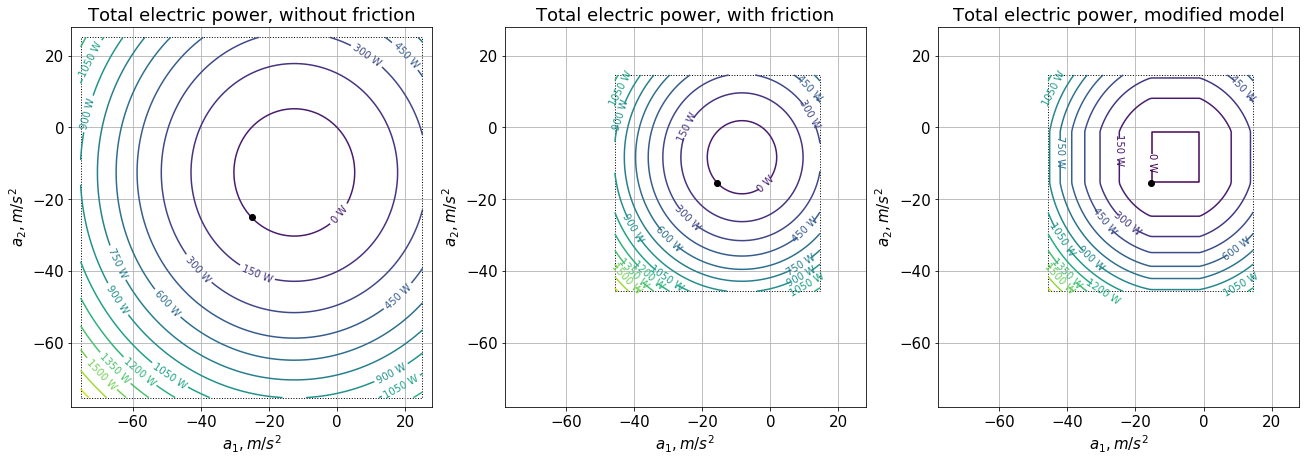
\includegraphics[width=1\linewidth]{power_from_w1_w2}
	\captionof{figure}{power as function of acceleration, moving in $w_1$ and $w_2$}
	\label{fig:power_from_w1_w2}
\end{figure}

Again, we can observe that the envelope remains unchanged in size and centered in the zero voltage point for the three graphs.

In the modified model, we can observe that the effect of degeneration into straight lines now applies for both axes: in the range of $a_1$ where power of motors 1 and 4 is zero, lines are horizontal, while in the range of $a_2$ where power of motors 2 and 3 is zero, lines are vertical. In the area in which both happen at the same time, we have a rectangle where power spent is zero.

\section*{Conclusions}

Las conclusiones están por concluir. Cuando concluyamos, las conclusiones serán concluidas y dejarán de estar inconclusas.
% Your references go at the end of the main text, and before the
% figures.  For this document we've used BibTeX, the .bib file
% scibib.bib, and the .bst file Science.bst.  The package scicite.sty
% was included to format the reference numbers according to *Science*
% style.


%\bibliography{scibib}

%\bibliographystyle{Science}



% Following is a new environment, {scilastnote}, that's defined in the
% preamble and that allows authors to add a reference at the end of the
% list that's not signaled in the text; such references are used in
% *Science* for acknowledgments of funding, help, etc.

%\begin{scilastnote}
%\item We've included in the template file \texttt{scifile.tex} a new
%environment, \texttt{\{scilastnote\}}, that generates a numbered final
%citation without a corresponding signal in the text.  This environment
%can be used to generate a final numbered reference containing
%acknowledgments, sources of funding, and the like, per {\it Science\/}
%style.
%\end{scilastnote}




% For your review copy (i.e., the file you initially send in for
% evaluation), you can use the {figure} environment and the
% \includegraphics command to stream your figures into the text, placing
% all figures at the end.  For the final, revised manuscript for
% acceptance and production, however, PostScript or other graphics
% should not be streamed into your compliled file.  Instead, set
% captions as simple paragraphs (with a \noindent tag), setting them
% off from the rest of the text with a \clearpage as shown  below, and
% submit figures as separate files according to the Art Department's
% instructions.


%\clearpage

%\noindent {\bf Fig. 1.} Please do not use figure environments to set
%up your figures in the final (post-peer-review) draft, do not include graphics in your
%source code, and do not cite figures in the text using \LaTeX\
%\verb+\ref+ commands.  Instead, simply refer to the figure numbers in
%the text per {\it Science\/} style, and include the list of captions at
%the end of the document, coded as ordinary paragraphs as shown in the
%\texttt{scifile.tex} template file.  Your actual figure files should
%be submitted separately.



\end{document}




















